To verify this methodology, two magnetic configurations are considered. In the first configuration, two cube magnets are arranged in repulsion, with one vertically above the other. The force between them is calculated as they move apart. The second configuration is similar, but the magnets do not move apart. Instead, one magnet is rotated while the force and torque on it are calculated. In addition, the magnetic field is calculated across the plane between the centres of the magnets. In this section, finite element simulations are used to verify both magnetic configurations with varying magnetic permeability.

\subsection{Magnets in repulsion}\label{sec:p4verification:magnetsRepulsion}
This section will analyse the magnetic system depicted in Figure \ref{fig:p4cubeMagnetsRepulsion} using various magnetic materials of varying permeabilities, with finite element simulations performed to verify the results obtained. In addition, the accuracy of approximating \(\mu_r = 1\) will be examined.

Consider the cube permanent magnets in Figure \ref{fig:p4cubeMagnetsRepulsion}. These magnets have a side length of \(l\) units, are separated by a distance \(d\), and are modelled with a relative permeability greater than unity, \(\mu_r > 1\). Specifically, these magnets are first modelled as neodymium magnets (\(\mu_r = 1.05\)), before being modelled as hard ferritic magnets (\(\mu_r = 1.2\)), and finally as alnico magnets (\(\mu_r = 3\)). Due to their relative permeabilities being greater than unity, each magnet slightly demagnetises itself. In addition, the magnets are in repulsion, so each magnet slightly demagnetises the other. This leads to a weaker repulsion force than expected.
\begin{figure}
	\centering
	\begin{tikzpicture}

% Set up coordinates of vertices
\coordinate(toptl) at (-1,3);
\coordinate(toptr) at (1,3);
\coordinate(topbl) at (-1,1);
\coordinate(topbr) at (1,1);
\coordinate(bottl) at (-1,0);
\coordinate(bottr) at (1,0);
\coordinate(botbl) at (-1,-2);
\coordinate(botbr) at (1,-2);

% Draw magnets
\draw (toptl) -- (toptr) -- (topbr) -- (topbl) -- cycle;
\draw (bottl) -- (bottr) -- (botbr) -- (botbl) -- cycle;

% Draw magnetisation vectors
\draw[->,thick] (0,2.5) -- (0,1.5);
\draw[->,thick] (0,-1.5) -- (0,-0.5);
\node(Mtop) at (0.5,2) {\(\mathbf{B}_{r\text{,top}}\)};
\node(Mbot) at (0.5,-1) {\(\mathbf{B}_{r\text{,bot}}\)};

% Draw dimensions
\draw[<->] (2,3) -- (2,1);
\node(lsidetop) at (2.3,2) {\(l\)};
\draw[<->] (-2,1) -- (-2,0);
\node(d) at (-1.7,0.5) {\(d\)};
\draw[<->] (2,0) -- (2,-2);
\node(lsidebot) at (2.3,-1) {\(l\)};
\draw[<->] (-1,-3) -- (1,-3);
\node(lunder) at (0,-2.8) {\(l\)};

\end{tikzpicture}
	\caption{Two cube magnets with side length \(l\) arranged in repulsion. The magnets are separated by a distance \(d\) and the force between them is calculated for varying separation distance \(d\).}
	\label{fig:p4cubeMagnetsRepulsion}
\end{figure}

To verify the work presented in this paper, the force between these magnets was calculated at a range of separation distances \(d\) in MATLAB R2020b (MathWorks, Inc., Natick, MA, USA) code and a finite element simulation using the Maxwell package in ANSYS Electronics Desktop 2018.0 (ANSYS, Inc., Berkeley, CA, USA)\footnote{When implementing the cubes in MATLAB and ANSYS Maxwell, a side length of 10mm was used. However, it should be noted that the methodology outlined in this chapter is dimensionless and any side length may be used with equivalent results.}. In addition, the force associated with a relative permeability of unity was calculated using the equations presented by \textcite{Akoun1984} to assess the modelling accuracy of assuming unity relative permeability. The methodology presented in this paper was applied to a surface mesh with approximately 6,000 triangular elements. In contrast, 25 passes of automatic mesh refinement were performed in ANSYS Maxwell, resulting in approximately 58,000 tetrahedral elements with quadratic shape functions, with approximately 4,500 elements per magnet and 49,000 in the air gap between and around the magnets. The percentage energy error and number of mesh elements for \(d = 0.5\) at each pass shown in Figure \ref{fig:p4repulseConvergence}. The forces are nondimensionalised by the permeability of a vacuum \(\mu_0\), the characteristic length \(l\), and the remanence magnetisations \(B_{r,\text{top}}\) and \(B_{r,\text{bot}}\),
\begin{equation}\label{eqn:p4forceNormalisation}
	\hat{F} = \frac{\mu_0}{l^2 B_{r\text{,top}} B_{r,\text{bot}}} F \text{,}
\end{equation}
and are displayed in Figure \ref{fig:p4cubeMagnetForces}. As can be seen, the finite element results converge and are in strong agreement with the results from this work. This indicates accurate results can be obtained from the methodology presented here.
%\begin{figure}
%    \centering
%    \includegraphics[width=0.5\linewidth]{p4/p4FIG3}
%    \vspace{-4mm}\caption{The mesh generated by ANSYS Maxwell after 25 passes of automatic mesh refinement for the magnetic configuration shown in Figure \ref{fig:p4cubeMagnetsRepulsion}. This mesh uses approximately 58,000 tetrahedral elements with quadratic shape functions, with approximately 4,500 elements per magnet and 49,000 elements in the region between and around the magnets.}
%    \label{fig:p4cubeMesh}
%\end{figure}
\begin{figure}
    \centering
    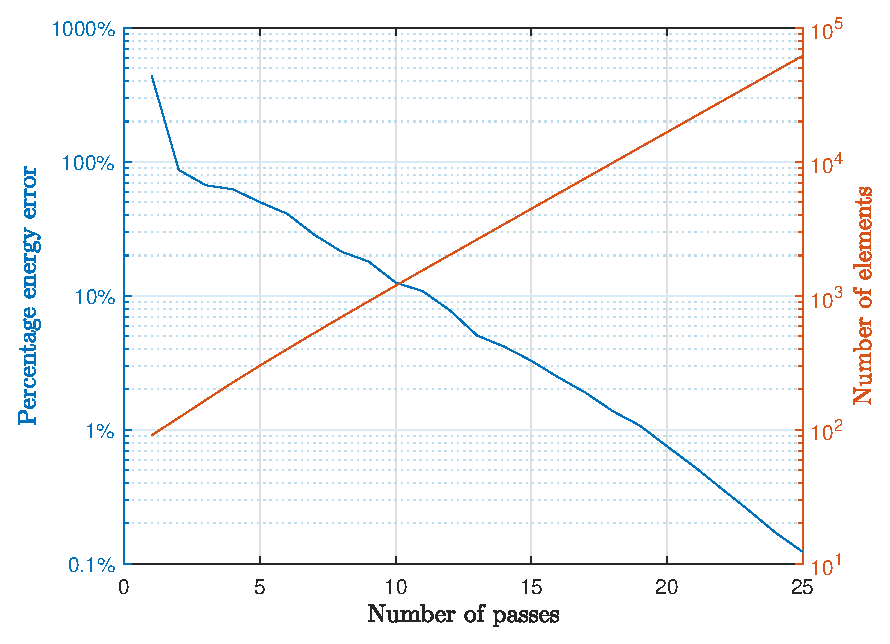
\includegraphics[width=0.8\textwidth]{p4/p4FIG4}
    \caption{Percentage energy error and number of tetrahedral elements in the ANSYS Maxwell simulation for \(d = 0.5\) as the number of passes of automatic mesh generation is increased.}
    \label{fig:p4repulseConvergence}
\end{figure}
\begin{figure}
	\centering
	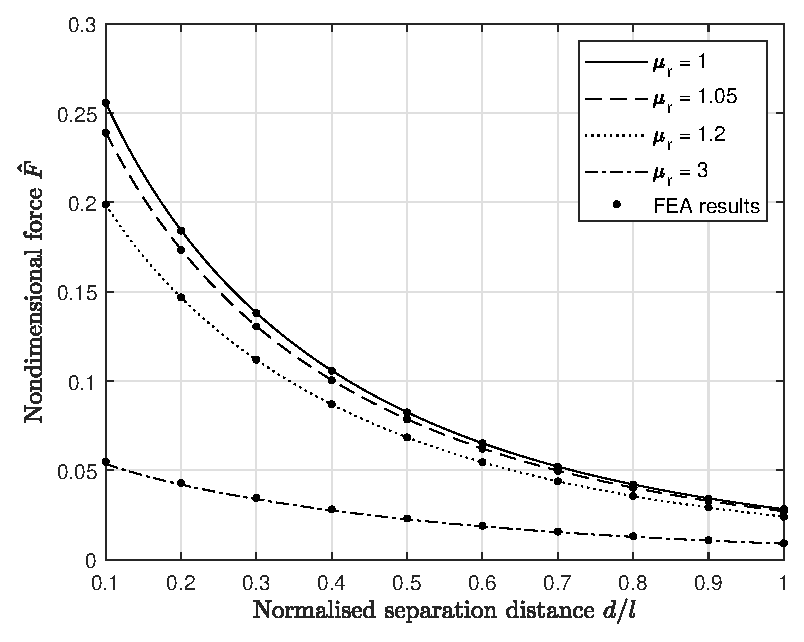
\includegraphics[width=0.8\linewidth]{p4/p4FIG5}
	\caption{Nondimensionalised force between the two magnets in Figure \ref{fig:p4cubeMagnetsRepulsion} for \(\mu_r = 1\) (calculated using \cite{Akoun1984}), \(\mu_r = 1.05\), \(\mu_r = 1.2\), and \(\mu_r = 3\). The forces calculated using the methodology presented in this paper are denoted with lines, with finite element simulations represented with large dots. The methodology presented above is in strong agreement with the finite element simulations, indicating correct force results.}
	\label{fig:p4cubeMagnetForces}
\end{figure}

In this simple repulsion configuration, it can be seen in Figure \ref{fig:p4cubeMagnetForces} that modelling neodymium magnets with \(\mu_r = 1\) overestimates the force by at least 4\%. While this is a nontrivial error, it is often accurate enough for preliminary designs. However, more permeable magnetic materials may give considerably larger errors. For this configuration, modelling hard ferritic magnets and alnico magnets with \(\mu_r = 1\) overestimates the force by at least 17\% and 170\% respectively. Thus, consideration of relative permeability in magnetostatic analysis is of high importance in electromagnetic design.

\subsection{Rotated magnets}
To verify the calculation of torque, a similar example is presented. Two cuboidal magnets, shown in Figure \ref{fig:p4cubeMagnetsRotated}, are positioned with a distance of \(3l/2\) between their centres. Initially, both magnets are parallel and magnetised along the positive vertical direction. The bottom magnet is rotated about its centre, and the force and torque on the magnet evaluated as it is rotated. The forces are nondimensionalised using Equation (\ref{eqn:p4forceNormalisation}) and the torques nondimensionalised by
\begin{equation}
	\hat{T} = \frac{\mu_0}{l^3 B_{r\text{,top}} B_{r,\text{bot}}} T \text{.}
\end{equation}
In addition, finite element simulations were conducted to examine error in the solutions found using this methodology. After 25 passes, the finite element mesh was similar to that obtained in Section \ref{sec:p4verification:magnetsRepulsion}, using approximately 58,000 tetrahedral elements, with approximately 4,500 elements per magnet and 49,000 elements in the region between and around the magnets. The percentage energy error and number of tetrahedral elements for \(\theta =\ \)\ang{60} at each pass is shown in Figure \ref{fig:p4rotateConvergence}, indicating convergence in the simulations. The torque results are plotted in Figure \ref{fig:p4cubeMagnetRotatedTorquex}, with the force results in Figures \ref{fig:p4cubeMagnetRotatedForcey} and \ref{fig:p4cubeMagnetRotatedForcez}.
\begin{figure}
	\centering
	\input{p4/p4FIG6}
	\caption{Two cube magnets with a side length of \(l\) maintaining a constant distance of \(3l/2\) between their centres. The force and torque on the bottom magnet is calculated as it is rotated an angle \(\theta\) about its centre.}
	\label{fig:p4cubeMagnetsRotated}
\end{figure}
\begin{figure}
    \centering
    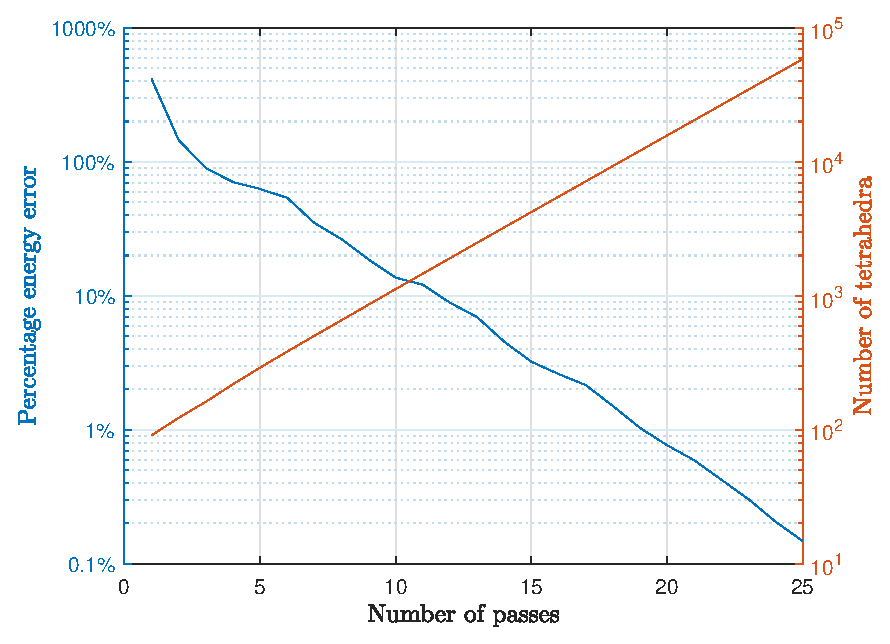
\includegraphics[width=0.8\linewidth]{p4/p4FIG7}
    \caption{Percentage energy error and number of tetrahedral elements in the ANSYS Maxwell simulation for \(\theta =\ \)\ang{60} as the number of passes of automatic mesh generation is increased.}
    \label{fig:p4rotateConvergence}
\end{figure}
\begin{figure}
	\centering
	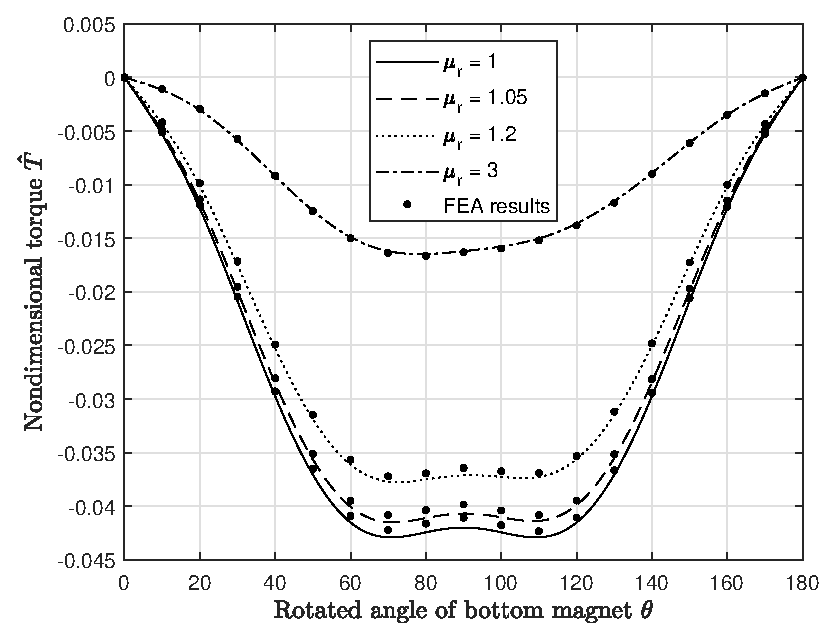
\includegraphics[width=0.8\linewidth]{p4/p4FIG8}
	\caption{Nondimensional torque on the bottom magnet about the axis of rotation of the magnet as it rotates for varying relative permeabilities \(\mu_r\). Finite element results are depicted with large dots, indicating some agreement with the results using the above methodology, with the FEA results being approximately 2\% smaller in magnitude for low permeabilities.}
	\label{fig:p4cubeMagnetRotatedTorquex}
\end{figure}
\begin{figure}
	\centering
	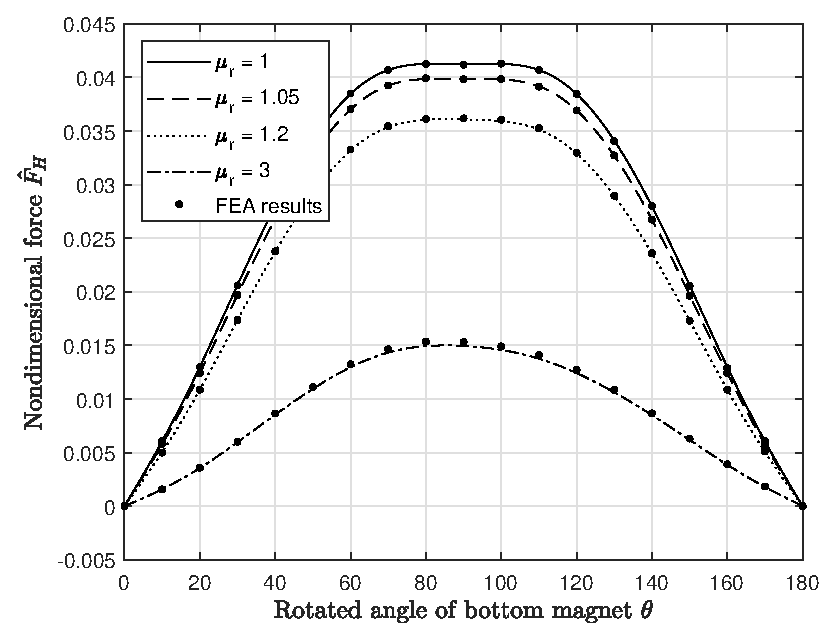
\includegraphics[width=0.8\linewidth]{p4/p4FIG9}
	\caption{Nondimensional horizontal force \(F_H\) on the bottom magnet as it rotates for varying relative permeabilities \(\mu_r\). Finite element results are depicted using large dots, indicating strong agreement with the results using the above methodology.}
	\label{fig:p4cubeMagnetRotatedForcey}
\end{figure}
\begin{figure}
	\centering
	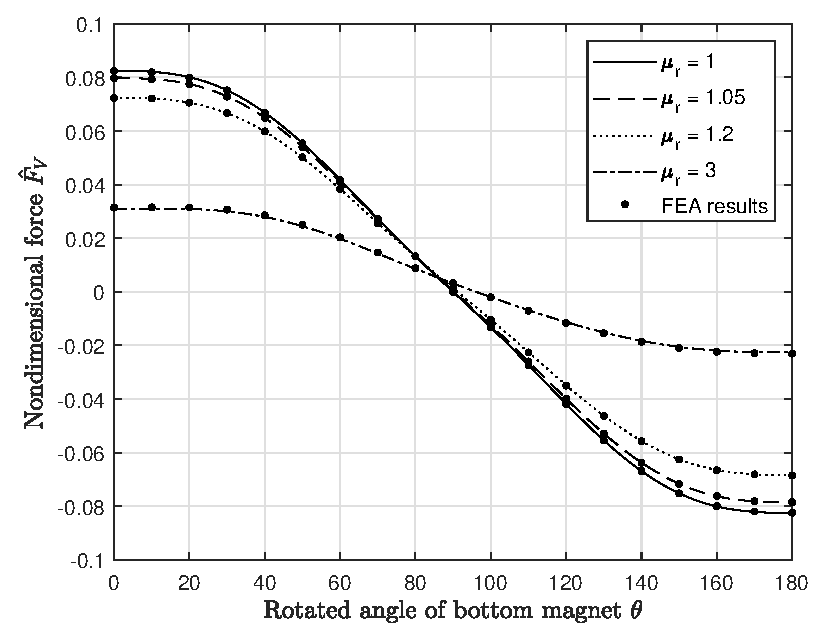
\includegraphics[width=0.8\linewidth]{p4/p4FIG10}
	\caption{Nondimensional vertical force \(F_V\) on the bottom magnet as it rotates for varying relative permeabilities \(\mu_r\). Finite element results are depicted using large dots, indicating strong agreement with the results using the above methodology.}
	\label{fig:p4cubeMagnetRotatedForcez}
\end{figure}
Figures \ref{fig:p4cubeMagnetRotatedTorquex}, \ref{fig:p4cubeMagnetRotatedForcey}, and \ref{fig:p4cubeMagnetRotatedForcez} show that the results obtained match closely with the finite element data. A small error between the estimated and FEA force results can be seen, with a larger error between the estimated and FEA torque results. To determine the source of this error, a special case of this configuration was used by setting \(\theta =\ \)\ang{90} and \(\mu_r = 1\). Since the magnets have parallel faces and a relative permeability of unity in this particular case, equations published by \textcite{Akoun1984} and \textcite{Janssen2010} can be used to calculate the exact force and torque respectively. The exact force in the horizontal direction and torque about the axis of rotation were calculated and compared to the results obtained using the methodology in this paper and finite element results, and are shown in Table \ref{tab:p4analyticTorque}.
\begin{table*}
    \centering
    \begin{tabular}{l|cc|cc}
    Method & $\hat F_H$ & Error & $\hat T$ & Error \\
    \hline
    Exact [4], [8] & $-0.04127$ & --- & $-0.04200$ & --- \\
    This work & $-0.04126$ & $0.02\%$ & $-0.04201$ & $0.24\%$ \\
    FEA & $-0.04120$ & $0.17\%$ & $-0.04107$ & $2.20\%$ \\
    \end{tabular}
    \caption{Nondimensional horizontal force \(\hat{F}_H\) and torque about the axis out of the page \(\hat{T}\) on the bottom magnet in Figure \ref{fig:p4cubeMagnetsRotated} at an angle of \ang{90} with both magnets having a relative permeability of \(\mu_r = 1\). The work presented here uses approximately 6,000 triangular surface elements, whereas the finite element simulations use approximately 58,000 tetrahedral volume elements. The work presented here has a considerably smaller percentage error than the finite element results when compared to the exact analytic results \cite{Akoun1984,Janssen2010}, indicating high accuracy of the work presented in this paper.}
    \label{tab:p4analyticTorque}
\end{table*}
It can be seen that for both force and torque, the results obtained using this methodology are considerably more accurate than the finite element results, with a percentage error almost ten times smaller. It appears that the finite element results are underestimating the force and torque, which may explain the discrepancy in Figures \ref{fig:p4cubeMagnetRotatedTorquex}, \ref{fig:p4cubeMagnetRotatedForcey}, and \ref{fig:p4cubeMagnetRotatedForcez}.

Interestingly, Figures \ref{fig:p4cubeMagnetRotatedTorquex}, \ref{fig:p4cubeMagnetRotatedForcey}, and \ref{fig:p4cubeMagnetRotatedForcez} show asymmetry when \(\mu_r \neq 1\). This is particularly visible in Figure \ref{fig:p4cubeMagnetRotatedTorquex} when \(\mu_r = 3\) between \(\theta =\ \)\ang{60} and \(\theta =\ \)\ang{120}, but this asymmetry occurs in all three plots and becomes more apparent as \(\mu_r\) is increased. This asymmetry is a result of the magnets producing fields which either strengthen or weaken the magnetisation of the other. When \(\theta <\ \)\ang{90}, the vertical component of the net field produced by the bottom magnet on the surface of the top magnet is in the same direction as \(\mathbf{B}_{r\text{,top}}\), thus strengthening the magnetisation of the top magnet. In the same way, the top magnet produces a field which strengthens the magnetisation of the bottom magnet. However, when \(\theta >\ \)\ang{90}, the opposite is true: Each magnet produces a field which weakens the magnetisation of the other magnet. Thus, each magnet strengthens the magnetisation of the other for \(\theta <\ \)\ang{90} and weakens the magnetisation of the other for \(\theta >\ \)\ang{90}, resulting in an asymmetry across \(\theta =\ \)\ang{90}, with a smaller magnitude of force and torque on the right side of each plot and a larger magnitude on the left.

In addition to verifying the force and torque, the magnetic field calculation is verified using the magnetic configuration in Figure \ref{fig:p4cubeMagnetsRotated} with \(\theta =\ \)\ang{90} and \(\mu_r = 3\) (as seen in Figure \ref{fig:p4cubeMagnetRotatedImage}). The magnetic field strength was calculated on the plane between the two magnets using the methodology in Section \ref{sec:p4magneticField} and nondimensionalised by the remanence magnetisation \(B_r\). In addition, finite element simulations were conducted on the same system using ANSYS Maxwell. The magnetic field strength computed using Section \ref{sec:p4magneticField} is plotted in Figure \ref{fig:p4cubeMagnetRotatedField}, along with the magnetic field strength generated by finite element simulations. The error is negligible, with a maximum error of 0.3\% of the remanence magnetisation, indicating the methodology used is calculating magnetic fields accurately.
\begin{figure}
	\centering
	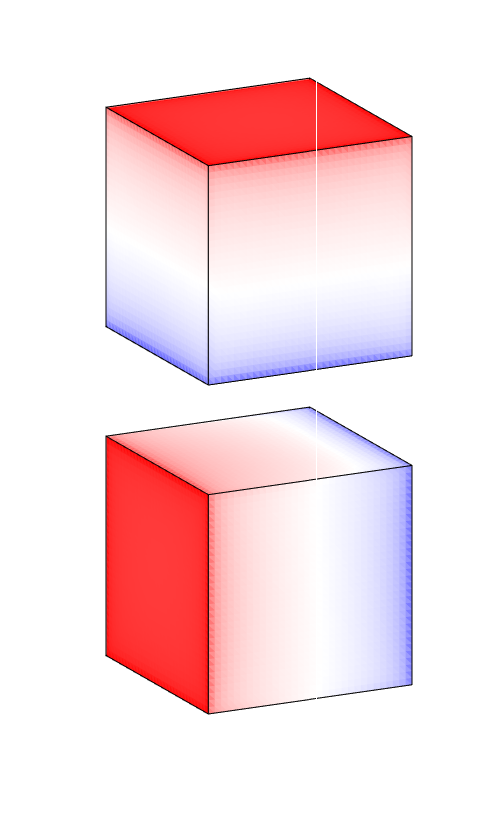
\includegraphics[width=0.55\linewidth]{p4/p4FIG11}
	\caption{The surface charge densities of the magnets in Figure \ref{fig:p4cubeMagnetsRotated} when \(\theta =\ \)\ang{90} and \(\mu_r = 3\). Due to the relatively large permeability, the top surface of the bottom magnet has considerably more positive surface charges accumulating than negative charges.}
	\label{fig:p4cubeMagnetRotatedImage}
\end{figure}
\begin{figure}
	\centering
	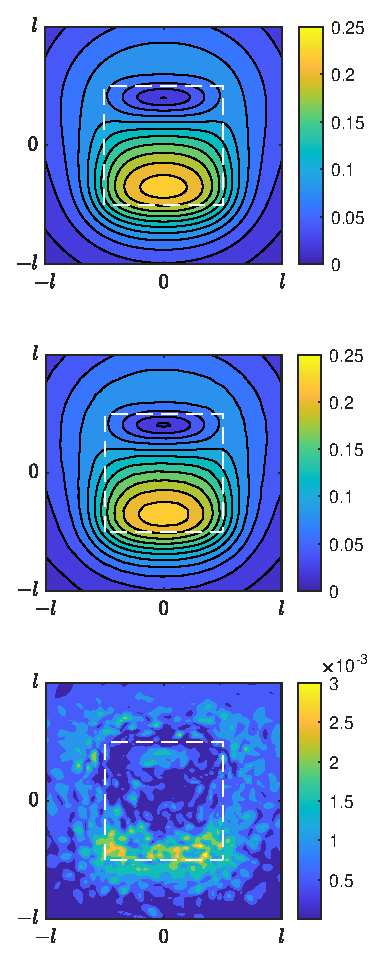
\includegraphics[width=0.5\linewidth]{p4/p4FIG12}
	\caption{The magnetic field strength \(\left| \mathbf{B} \right|\) normalised by \(B_r\) on the plane between the two magnets in Figure \ref{fig:p4cubeMagnetsRotated} when \(\theta =\ \)\ang{90}. The projections of the magnets onto the plane are displayed using white dashed lines. The field was calculated using the methodology in this paper (top) and finite element simulations (middle), with the absolute error between the two calculated (bottom). This shows strong agreement, with a maximum error of 0.3\% of the remanence magnetisation.}
	\label{fig:p4cubeMagnetRotatedField}
\end{figure}